\section{Mean Teacher for general improvement}
\label{sec:mean_teacher_general}

As described in \ref{sec:mean_teacher}, the mean teacher approach should enable us to utilize unlabeled data to improve the performance of our model.
To verify the effectiveness of this approach, the method is first tested on the Cityscapes dataset before it is applied to the vapour dataset.

In this experiment, the only concern is to improve the general performance of the model measured by the metrics described above. 
Further experiments will verify the effectiveness of the method for improving the generalization capabilities of the model on the vapour dataset.

\paragraph{Verification on Cityscapes} 

For the Cityscapes dataset training is done on images downsampled to a \qtyproduct{256 x 512}{\pixel} resolution. The initial learning rate is set to \num{1e-3} and the batch size to 16 containing 4 labeled and 12 unlabeled samples. The patience for the scheduler is set to 5 epochs and the reduction factor is set to \num{0.1}.
The weight of the consistency loss is ramped up to its maximum value of \num{1.0} over the first 15 epochs using a sigmoid ramp.
Consistency loss is calculated using the \emph{cross entropy loss} between the predictions of the student and the hard predictions of the teacher (meaning after applying \emph{argmax}).
The teacher is updated using an EMA with a decay $\alpha$ of \num{0.996}.

For the baseline model, the best results are achieved by using an initial learning rate of \num{1e-4} with a batch size of 16, a scheduler patience of 20 epochs and a reduction factor of \num{0.5}. 

The baseline model is trained on 100 labeled samples from the training set, while the mean teacher model is trained on the same 100 lableled samples plus all other samples from the training set as unlabeled samples.
A training epoch when using MT is considered to be finished when the model has seen all unlabeled samples once, with the labeled samples being seen as many times as necessary to fill the batch size. This means epochs for MT training contain considerably more samples than epochs for baseline training, which is why the patience value for baseline training is higher.

For the baseline model, the augmentation pipeline consists of a random \numproduct{224 x 224} crop, a random translation, scaling and rotation with a probability of \num{0.5}, a RGB-shift with a probability of \num{0.5} and a random variation of the image brightness and contrast with a probability of \num{0.5}.  

The augmentation pipeline for the MT training employs a different set of augmentations, since strong asymmetrical augmentations between teacher and student are important for the MT approach to properly function. For this, the augmentation pipeline is inspired by \Citeauthor{schererPseudoLabelNoiseSuppression2022}\cite{schererPseudoLabelNoiseSuppression2022}. It contains the same shift, scale, rotation and crop operations as the baseline augmentations, but also applies a strong dropout of \num{0.5} to the student model, as well as using a \emph{CowMask} technique to compose new samples by combining two images as well as their teacher predictions.
For this technique a mask such as the one shown in Figure \ref{fig:cowmask} is generated and applied to an image and its pseudo label. The same is done for a second image and its pseudo label with the inverted mask and both are combined.

Finally, the images are normalized using the mean and standard deviation of the ImageNet dataset in both baseline and MT training.

\begin{figure}[htbp]
    \centering
    \makebox[\textwidth][c]{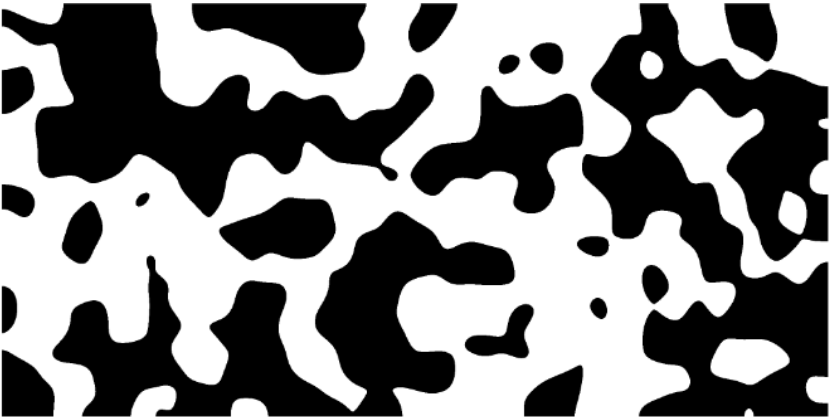
\includegraphics[width=0.4\textwidth]{images/Screenshot-20230221170853-829x417.png}}
    \vspace{0.1cm}
    \caption{Example for a cow mask used in the training process. The white areas mark regions that use the first image, while the black areas use the second image. From \cite{schererPseudoLabelNoiseSuppression2022}}
    \label{fig:cowmask}
\end{figure}

\paragraph{Results on Cityscapes}
With the MT approach, the model is able to achieve a mean IoU of \num{0.426} on the validation set, which is a significant improvement over the baseline model with a mean IoU of \num{0.349}.

However, this improvement is only achievable within a very small space of hyperparameters, as all training runs with different hyperparameters than described above yielded worse results than even the baseline model.

This deterioration in performance can likely be attributed to very poor pseudo label quality. As \citeauthor{schererPseudoLabelNoiseSuppression2022}\cite{schererPseudoLabelNoiseSuppression2022} discovered in their analysis of \emph{pseudo label filtering} techniques, pseudo labels with poor quality have a detrimental effect on final model performance.
Since the setup used in this thesis doesn't achieve very high performance on the Cityscapes dataset as is, even when using all labeled samples (mIoU of \num{0.475}), it stands to reason that label quality may hurt the training process if hyperparameters are suboptimal.

Nonetheless, the results of this experiment show that the MT approach is able to improve the performance of the model. With the supervised performance on the target dataset being signifcantly better than on the Cityscapes dataset, it is likely that the MT approach will be able to improve the performance of the model on the vapour dataset as well.

For a more comprehensive overview of training results, see Table \ref{tab:cityscapes_results_mt}.

\begin{table}[htbp]
    \centering
    \begin{tabular}{llllllllrr}
        \toprule
        \multicolumn{9}{l}{Cityscpapes Training}\\  
        \midrule
        Approach & \#lbls & lr & bsize & lrsf & lrsp & Dropout & $\alpha$ & Loss &
        mIoU \\
        \midrule 
        Baseline & all & $0.0001$ & $16$ & $0.5$ & $10$ & - & - & $0.216$ & $0.475$ \\
        MT & 100 & $0.001$ & $16$ & $0.1$ & $5$ & \num{0.5} & \num{0.996} & $0.644$ & $\mathbf{0.426}$ \\
        MT & 100 & $0.001$ & $16$ & $0.1$ & $5$ & \num{0.4} & \num{0.996} & $0.559$ & $0.412$ \\
        Baseline & 100 & $0.0001$ & $16$ & $0.5$ & $30$ & \num{0.2} & - & $0.444$ & $0.349$ \\
        Baseline & 100 & $0.0001$ & $16$ & $0.5$ & $30$ & - & - & $0.469$ & $0.331$ \\
        \bottomrule
    \end{tabular}
    \vspace{0.1cm}
    \caption{The best training results of the Mean Teacher approach on the Cityscapes dataset, as well as the supervised baseline performance along with important hyperparameters. For abbreviations refer to Table \ref{tab:abbreviations}.}
    \label{tab:cityscapes_results_mt}
\end{table}

\paragraph{Setup on vapour dataset}
The training setup for the vapour dataset is very similar to the Cityscapes setup, with the images being split in half along the vartical and horizontal axis and these 4 segments being used as seperate samples. The decision to split the images instead of resizing them was made because the relevant objects in the images are already quite small, so resizing them might make it impossible to detect some of them. This leaves us with \qtyproduct{640 x 512}{\pixel} images, which necessitated lowering the batch size to 12 for baseline training and 8 (2 labeled, 6 unlabeled) for MT training.
Learning rate was generally found to be optimal around \num{1e-3}.

Another difference in the setup is the augmentation pipeline, which is similar to the Cityscapes pipeline, but replaces the RGB-shift with gaussian noise, since the vapour dataset contains greyscale images. The gaussian noise might also be able to mimic some of the noise the camera produces, so it seems like an adequate replacement.
Furthermore, we also explore using \emph{CutMix}\cite{yunCutMixRegularizationStrategy2019} for mixing pseudo labels instead of the CowMask technique used for Cityscapes. 
CutMix cuts a rectangular region of the image instead of the varying sizes of blobs in the CowMask technique.
The reason this may be more suitable to the vapour dataset is that the objects in the images are generally quite small, so the CowMask technique, which masks generally smaller regions might not be effective in combining relevant features from the two images. On Cityscapes, CutMix was not attempted since \Citeauthor{schererPseudoLabelNoiseSuppression2022}\cite{schererPseudoLabelNoiseSuppression2022} already concluded that the CowMask technique was superior.

\paragraph{Results on vapour dataset}

